% =====================================================================
% Draft for Computers & Fluids (Elsevier, elsarticle class).
%
% Compile: pdflatex main && pdflatex main
%
% BIBLIOGRAPHY WARNING.  The reference list was assembled from search
% results and memory.  Entries marked [VERIFY] have year, volume or page
% numbers I could not confirm and MUST be checked against the sources
% before submission.
% =====================================================================
\documentclass[preprint,12pt,3p]{elsarticle}

\usepackage{amsmath,amssymb,amsthm}
\usepackage{booktabs}
\usepackage{siunitx}
\usepackage{graphicx}
\usepackage{pgfplots}
\pgfplotsset{compat=1.18}
\usepgfplotslibrary{groupplots}
\usepackage[colorlinks=true,allcolors=blue]{hyperref}

\newtheorem{theorem}{Theorem}
\newtheorem{lemma}[theorem]{Lemma}
\newtheorem{corollary}[theorem]{Corollary}
\theoremstyle{remark}
\newtheorem{remark}[theorem]{Remark}

\newcommand{\grade}[2]{\left\langle #1 \right\rangle_{#2}}
\newcommand{\eps}{\varepsilon_3}
\newcommand{\dd}{\mathrm{d}}
\newcommand{\bx}{\mathbf{x}}
\newcommand{\bu}{\mathbf{u}}
\newcommand{\br}{\mathbf{r}}
\newcommand{\bn}{\mathbf{n}}
\newcommand{\bG}{\mathbf{G}}
\newcommand{\bomega}{\boldsymbol{\omega}}
\newcommand{\balpha}{\boldsymbol{\alpha}}
\newcommand{\bgamma}{\boldsymbol{\gamma}}

\journal{Computers \& Fluids}

\begin{document}

\begin{frontmatter}

\title{The discarded grade: a cost-free solenoidality diagnostic\\
for vortex and panel methods}

\author{Onur Tuncer}
\ead{onur.tuncer@itu.edu.tr}
\address{Department of Aeronautical Engineering, Istanbul Technical University, Istanbul, Turkey}

\begin{abstract}
The discrete vorticity field of a three-dimensional vortex method is not
solenoidal. The error is generated by the discretisation, amplified by
stretching, and corrected in practice by relaxation or projection schemes
applied on a fixed schedule --- because measuring it costs either a grid or a
second summation, so its growth is inferred from stability rather than
observed. We show that the quantity is already being computed and discarded.
Writing the velocity as a Clifford-algebra convolution, an established
reformulation in which source density and vorticity are the scalar and bivector
grades of one flow charge, the geometric product yields a grade-3 term
alongside the velocity that the classical cross-product formulation never
forms. We prove that this term $\eps$ satisfies $\nabla^2\eps =
\nabla\cdot\bomega$: it is the Newtonian potential of the vorticity divergence.
Integrated in closed form along a straight filament it telescopes, so a closed
filament of constant circulation cancels to round-off at any resolution and any
core radius, giving a diagnostic that measures topology rather than resolution.
Scalar measures contribute nothing to grade 3, so the residual isolates the
vortex system automatically in fields of arbitrary source content. Adding it to
an existing solver costs one inner product of two vectors already in registers
--- three multiplies and two adds per interaction --- with no grid, no auxiliary
kernel and no change of formulation; under fast summation it emerges from the
same local expansion as the velocity and remains $O(1)$ per evaluation. In a
vortex lattice it detects a $0.01\%$ circulation-conservation error twelve
orders of magnitude above its noise floor while the lift coefficient moves by
$\num{2.7e-5}$; in a wing--body solver it reports on the wake while several
hundred source panels contribute nothing; and on an evolving particle ring it
separates two standard stretching discretisations by ten orders of magnitude
from a common machine-zero start, while the conservation check normally relied
upon stays at machine precision and detects nothing. We are explicit about what
the diagnostic does not do: a vanishing residual certifies that a discrete
vortex system is realisable, not that it is accurate.
\end{abstract}

\begin{keyword}
vortex methods \sep solenoidality \sep a posteriori diagnostics \sep
vortex particle method \sep panel methods \sep geometric algebra
\end{keyword}

\end{frontmatter}

% =====================================================================
\section{Introduction}
\label{sec:intro}

Three-dimensional vortex methods carry a defect that has been understood for
decades and is rarely measured. The vorticity field represented by a set of
particles or filaments is not solenoidal. The exact equations preserve
$\nabla\cdot\bomega=0$; a particle discretisation does not, and the initial
error is amplified by the stretching term, degrading accuracy and stability in
long-time and high-Reynolds-number simulation \cite{cottet2000,winckelmans1993}.

The response has been corrective rather than diagnostic. Relaxation schemes due
to Pedrizzetti \cite{pedrizzetti1992} and Winckelmans \cite{winckelmans1993}
realign particle strengths with the local vorticity; projection methods map the
field onto a divergence-free basis. These are applied by default in
contemporary solvers: the reformulated vortex particle method of Alvarez and
Ning \cite{alvarez2024} resolves stretching with the transposed scheme and
treats the divergence of the vorticity field with Pedrizzetti relaxation.

What is missing is a way to observe the error without paying for it. Evaluating
$\nabla\cdot\bomega$ directly requires a grid, or a second $O(N^2)$ summation
against a different kernel; measuring the deviation of a vortex field from the
nearest divergence-free field requires constructing that field. In consequence
the defect is suppressed rather than monitored, the strength and frequency of
the suppression are tuned by experience, and its effectiveness is inferred from
stability rather than measured.

This paper observes that the quantity is already being computed and thrown
away, and that recovering it costs a single inner product.

\subsection{Origin of the diagnostic}

Write the incompressible velocity field as a Clifford-algebra convolution. The
reformulation is not new. Representing vorticity as a bivector and casting the
Euler or Navier--Stokes system in geometric-algebra form is established
\cite{hestenes1984,doran2003,sugon2024}, and Clifford analysis has been applied
to fluid boundary value problems since the work of Gürlebeck and Sprößig
\cite{gurlebeck1997book,sprossig1997}. In the algebra $Cl(3,0)$ the velocity
satisfies the single first-order equation
\begin{equation}
  \nabla\bu = \nabla\cdot\bu + \nabla\wedge\bu = q + I\bomega ,
  \label{eq:field}
\end{equation}
and the Green's function of the vector derivative recovers the velocity by
grade projection, reproducing the classical source and Biot--Savart kernels as
the scalar and bivector parts of one product.

The product $\bG Q$ is, however, a multivector. Alongside the grade-1 part that
is the velocity it carries a grade-3 part,
$\grade{\bG Q}{3} = I(\bG\cdot\bomega)$, which no implementation retains
because the classical formulation, built on the cross product, never forms it.
This paper is about that discarded term.

\subsection{A note on adoption}

A reader is not asked to reformulate a solver in geometric algebra. The algebra
explains where the quantity comes from and why it has the properties it does,
but the result is a scalar accumulated by three multiplies and two adds inside
an existing Biot--Savart loop, as set out in Section~\ref{sec:implementation}.
Nothing else in an existing code need change.

\subsection{Contributions}

\begin{enumerate}
\item $\eps$ is the Newtonian potential of the vorticity divergence,
  $\nabla^2\eps = \nabla\cdot\bomega$ (Theorem~\ref{thm:C}), connecting the
  discarded grade to the defect described above.
\item Its discrete form carries no resolution floor
  (Theorem~\ref{thm:Bprime}): integrated exactly along straight segments the
  term telescopes, so a closed filament of constant circulation cancels
  identically at any number of segments and any core radius. The residual
  measures topology, not resolution.
\item It is blind to source content (Corollary~\ref{cor:blind}), so it operates
  unmodified inside source-dominated panel solvers.
\item It is free: one inner product of quantities already formed for the
  velocity, and $O(1)$ per evaluation under fast summation.
\item It detects what force-based and conservation-based checks cannot
  (Sections~\ref{sec:static}--\ref{sec:dynamic}).
\end{enumerate}

We also report, and do not overstate, an open question. Whether the diagnostic
can be used to improve relaxation practice is not settled here; two experiments
in opposite regimes give opposite signs, and Section~\ref{sec:relaxation}
identifies the resolution required to decide the matter, which lies beyond
direct summation.

% =====================================================================
\section{The velocity kernel}
\label{sec:kernel}

This section fixes notation and records the reformulation the rest of the paper
uses. Nothing in it is claimed as new; see
\cite{hestenes1984,doran2003,gurlebeck1997book,sugon2024}.

\subsection{Algebra}

Work in $Cl(3,0)$ over $\mathbb{R}^3$ with orthonormal basis $\{e_1,e_2,e_3\}$,
$e_ie_j+e_je_i = 2\delta_{ij}$, and unit pseudoscalar $I = e_1e_2e_3$ satisfying
$I^2=-1$ and commuting with everything. For vectors,
$\mathbf{a}\mathbf{b} = \mathbf{a}\cdot\mathbf{b}+\mathbf{a}\wedge\mathbf{b}$
with $\mathbf{a}\wedge\mathbf{b} = I(\mathbf{a}\times\mathbf{b})$. A bivector is
stored by its dual vector, $B = I\mathbf{w}$; in the cyclic basis
$\{e_{23},e_{31},e_{12}\}$ the components coincide.

\subsection{Flow charge and representation}

With $\nabla = e_i\partial_i$ the vector derivative, \eqref{eq:field} defines
the \emph{flow charge}
\begin{equation}
  Q := \nabla\bu = q + I\bomega ,
\end{equation}
a scalar-plus-bivector multivector whose grades are source density and
vorticity. Two conventions are fixed by the derivation rather than chosen:
$\nabla$ acts from the left, so the Green's function stands to the left of the
measure; and the bivector grade is $+I\bomega$, because that is what
$\nabla\wedge\bu$ produces.

The fundamental solution of the vector derivative is
\begin{equation}
  \bG(\br) = \frac{\br}{4\pi|\br|^3} = -\nabla\frac{1}{4\pi|\br|},
  \qquad \nabla\bG = \delta^3(\br),
  \label{eq:green}
\end{equation}
giving
\begin{equation}
  \bu(\bx) = \int \bG(\bx-\bx')\,Q(\bx')\,\dd V' ,
  \label{eq:rep}
\end{equation}
whose integrand decomposes by grade as
\begin{align}
  \grade{\bG Q}{1} &= q\,\bG + \bomega\times\bG , \label{eq:grade1}\\
  \grade{\bG Q}{3} &= I\,(\bG\cdot\bomega) . \label{eq:grade3}
\end{align}

Equation \eqref{eq:grade1} is the classical catalogue. With
$q\,\dd V\to\sigma\,\dd S$ it is the constant-source panel; with
$\bomega\,\dd V\to\bgamma\,\dd S$ the vortex sheet; with
$\bomega\,\dd V\to\Gamma\,\dd\boldsymbol{\ell}$ the Biot--Savart law; with
$\bomega\,\dd V\to\balpha$ a vortex particle; and a constant-strength doublet
panel is its edge ring with $\Gamma=\mu$.

\begin{remark}[Mollification]
\label{rem:moll}
Regularised cores belong to $\bG$, not to the kernel or any measure. Every blob
is a radial rescaling $\bG_\delta(\br) = s_\delta(|\br|)\br$ of the same vector,
and since $s_\delta$ is scalar it commutes with grade projection:
$\grade{\bG_\delta Q}{k} = s_\delta\grade{\bG Q}{k}$ for every $k$. Smoothing is
therefore orthogonal to everything below. We use the Rosenhead--Moore blob
$s_\delta = [4\pi(d^2+\delta^2)^{3/2}]^{-1}$ where a closed-form line integral
is needed, and the Gaussian otherwise.
\end{remark}

% =====================================================================
\section{The discarded grade}
\label{sec:theory}

Equation \eqref{eq:grade3} is generally non-zero pointwise. Write
\begin{equation}
  \eps(\bx) := \int \bG(\bx-\bx')\cdot\bomega(\bx')\,\dd V'
  \label{eq:eps}
\end{equation}
for its pseudoscalar coefficient. It has the dimensions of velocity.

\subsection{The residual is the potential of the divergence}

\begin{theorem}[Divergence potential]
\label{thm:C}
For vorticity of compact support,
\begin{equation}
  \eps(\bx) = -\int \frac{(\nabla\cdot\bomega)(\bx')}{4\pi|\bx-\bx'|}\dd V' ,
  \qquad\text{hence}\qquad \nabla^2\eps = \nabla\cdot\bomega .
\end{equation}
\end{theorem}

\begin{proof}
Let $\phi(\bx,\bx') = 1/(4\pi|\bx-\bx'|)$, so that
$\nabla_{\bx'}\phi = (\bx-\bx')/(4\pi|\bx-\bx'|^3) = \bG(\bx-\bx')$ and
\eqref{eq:eps} reads $\int(\nabla_{\bx'}\phi)\cdot\bomega\,\dd V'$. Integrating
by parts,
\[
  \eps(\bx) = \oint \phi\,\bomega\cdot\bn\,\dd S'
            - \int \phi\,(\nabla'\!\cdot\bomega)\,\dd V' ,
\]
with the surface term vanishing for compactly supported $\bomega$. Applying
$\nabla^2_{\bx}$ and using $\nabla^2_{\bx}\phi = -\delta(\bx-\bx')$ gives the
second statement.
\end{proof}

The grade the classical formulation discards is therefore precisely the
Newtonian potential of the solenoidality defect: a smoothed, non-local measure
of $\nabla\cdot\bomega$ reporting its integrated effect on the velocity field
rather than a pointwise derivative.

\subsection{Closure of filaments and sheets}

\begin{theorem}[Helmholtz obstruction]
\label{thm:B}
$\eps$ vanishes identically for all field points if and only if the circulation
of every filament is constant along closed curves, and every sheet strength is
surface-solenoidal with edge circulation shed into bounding filaments.
\end{theorem}

\begin{proof}[Sketch]
Along a curve with unit tangent $\mathbf{t}$ and circulation $\Gamma$,
$\bG\cdot\mathbf{t} = (4\pi)^{-1}\dd(1/|\br|)/\dd s$, so the line integral of
\eqref{eq:eps} telescopes and vanishes on any closed curve of constant $\Gamma$.
For a sheet of strength $\bgamma$ on $S$,
$\int_S\bG\cdot\bgamma\,\dd S
 = \oint_{\partial S}(\bgamma/|\br|)\cdot\dd\boldsymbol{\ell}_\perp
 - \int_S(\nabla_S\!\cdot\bgamma)/|\br|\,\dd S$,
vanishing exactly when the sheet strength is surface-solenoidal and the edge
term is absorbed by shed filaments. These are Helmholtz's vortex theorems and
the wake-shedding condition.
\end{proof}

Grade projection $\grade{\cdot}{1}$ is thus not a notational convenience but a
licence, valid only when the vortex system is closed. Every vortex code assumes
this silently; retaining the grade makes the assumption a computable number.

\subsection{The discrete residual carries no floor}

A diagnostic whose zero is a quadrature-error floor cannot separate a broken
vortex system from an under-resolved one. The discrete form is sharp.

\begin{theorem}[Exact discrete closure]
\label{thm:Bprime}
Integrating \eqref{eq:eps} in closed form along a straight segment from
$\mathbf{a}$ to $\mathbf{b}$,
\begin{equation}
  \int_{\mathbf{a}}^{\mathbf{b}}\bG\cdot\bomega\,\dd\ell
  = \frac{\Gamma}{4\pi}\left[\frac{1}{|\bx-\mathbf{b}|}-\frac{1}{|\bx-\mathbf{a}|}\right],
  \label{eq:telescope}
\end{equation}
and identically under the Rosenhead--Moore mollifier with
$|\br|\mapsto\sqrt{|\br|^2+\delta^2}$. Hence for a closed polygonal filament of
constant circulation evaluated with exact segment integration, $\eps=0$ to
round-off for any number of segments and any core radius.
\end{theorem}

Exact segment integration is therefore a requirement of the method rather than
an optimisation: with midpoint quadrature the residual acquires an $O(h^2)$
floor (Table~\ref{tab:filament}) that would mask a genuine closure violation of
comparable size.

\begin{remark}
A regular polygon cancels the midpoint-quadrature residual by symmetry rather
than by closure. Validation must use an asymmetric curve.
\end{remark}

\subsection{Blindness to sources}

\begin{corollary}
\label{cor:blind}
Scalar measures contribute nothing to grade 3. In a mixed field
$Q = q + I\bomega$, $\eps$ depends on $\bomega$ alone.
\end{corollary}

This is immediate from \eqref{eq:grade3} and allows the diagnostic to be
embedded unchanged in a source-dominated problem, as Section~\ref{sec:mixed}
demonstrates.

% =====================================================================
\section{Implementation}
\label{sec:implementation}

\subsection{Adding it to an existing solver}

Let $\mathbf{g} = \bG_\delta(\bx-\bx')$ be the regularised kernel vector already
formed inside the velocity loop. Then
\begin{equation}
  \grade{\bG Q}{1} = q\,\mathbf{g} + \bomega\times\mathbf{g},
  \qquad
  \grade{\bG Q}{3} = \mathbf{g}\cdot\bomega ,
\end{equation}
so the diagnostic is accumulated by
\begin{verbatim}
    residual += dot(g, omega);   // 3 multiplies, 2 adds
\end{verbatim}
alongside the existing velocity accumulation. There is no additional kernel
evaluation, no square root, no transcendental, and no grid. Evaluating
$\nabla\cdot\bomega$ directly instead would require a second summation against
$\nabla\zeta_\delta$, a different radial power, at a cost comparable to the
velocity sum itself.

\subsection{Behaviour under fast summation}
\label{sec:fmm}

Since $\bG = -\nabla\phi$ with $\phi$ the Laplace kernel, \eqref{eq:rep} factors
as $\bu = -\nabla(\phi\star Q)$, where $\phi\star Q$ is componentwise: four
independent scalar Laplace convolutions. Both grades then follow from
differentiating the \emph{same} local expansion,
$\grade{\nabla\Psi}{1} = \nabla\Psi_0 + \nabla\cdot\Psi_2$ and
$\grade{\nabla\Psi}{3} = \nabla\wedge\Psi_2$, so the diagnostic remains $O(1)$
per evaluation at any problem size rather than degrading into a separate
$O(N\log N)$ pass.

We claim no reduction in the number of convolutions relative to a classical
treecode or fast multipole implementation. The classical formulation also
computes one scalar potential and a three-component vector potential, and
already places all elements in a single tree. The claim is only that the
residual is free once the velocity is being computed.

\begin{remark}[Free in cost; accuracy set by the velocity]
\label{rem:accuracy}
Under an \emph{approximate} evaluation the residual inherits the velocity's
\emph{absolute} error, and since $|\eps|\ll|\bu|$ on a nearly solenoidal field
its relative accuracy is correspondingly worse. A Cartesian treecode on the
volumetric ring of Section~\ref{sec:relaxation} makes the relation concrete:

\begin{center}
\begin{tabular}{ccccc}
\toprule
order & $\theta$ & velocity rel. & $\eps$ rel. & $\eps$ err. / RMS speed \\
\midrule
2 & 0.3 & \num{2.34e-4} & \num{4.99e-1} & \num{2.17e-4} \\
4 & 0.3 & \num{2.17e-5} & \num{3.39e-2} & \num{1.48e-5} \\
6 & 0.3 & \num{1.34e-6} & \num{1.88e-3} & \num{8.17e-7} \\
\bottomrule
\end{tabular}
\end{center}

The last column tracks the velocity's relative error at every order, confirming
that the residual is resolvable only down to about (velocity relative error)
$\times|\bu|$. This is a property of approximate evaluation rather than an
obstacle: raising the expansion order drives both down together, and at sixth
order the residual is recovered to better than $0.2\%$. An implementation
seeking to monitor a small defect must therefore choose its expansion order
from the defect it wishes to resolve, not from the accuracy it needs in the
velocity. No result in this paper is affected, all being direct sums, but the
relation bounds what fast summation delivers and we state it rather than leave
it to be discovered.
\end{remark}

\subsection{Two implementation traps}

Filaments must use the closed form \eqref{eq:telescope} rather than point
quadrature; an implementation using midpoint quadrature obtains a diagnostic
that appears to work and silently does not.

Separately, panel codes evaluating the solid angle by the Van
Oosterom--Strackee formula \cite{vanoosterom1983} must treat the in-plane case
explicitly. At a point in a panel's own plane the denominator turns negative
inside the triangle and $\operatorname{atan2}$ returns $\pm2\pi$ instead of the
principal value $0$, with the $\pm1/2$ jump then added by the caller. A code
with this error still produces plausible surface speeds, because the normal
component is projected out, and fails only when the Neumann residual is
checked.

% =====================================================================
\section{Verification}
\label{sec:verification}

All results come from a dependency-free C++20 implementation; an independent
Python implementation reproduces the deterministic rows exactly. Verification
uses a brute-force eight-component $Cl(3,0)$ product engine sharing no code path
with the closed-form grade expressions, together with refined quadrature,
rather than algebraic restatements of the same formulae.

\begin{table}[htbp]
\centering
\caption{Verification of the kernel and its grade projections. Rows 1--2 are the
substantive checks; rows 3--5 confirm that the element constructors reduce to
the classical formulae.}
\label{tab:verify}
\begin{tabular}{lr}
\toprule
Check & Max.\ error \\
\midrule
$\grade{\bG Q}{1}$ vs.\ independent $Cl(3,0)$ product & \num{2.22e-16} \\
$\grade{\bG Q}{3}$ vs.\ independent $Cl(3,0)$ product & \num{0.0} \\
Source element vs.\ $\sigma\br/4\pi|\br|^3$ & \num{4.44e-16} \\
Filament element vs.\ Biot--Savart & \num{5.55e-17} \\
Sheet element vs.\ $\bgamma\times\br/4\pi|\br|^3$ & \num{1.11e-16} \\
Mollification commutes with grade projection & \num{5.55e-17} \\
Exact segment vs.\ refined quadrature (relative) & \num{4.08e-9} \\
Panel integral vs.\ refined quadrature (relative) & \num{9.80e-7} \\
\bottomrule
\end{tabular}
\end{table}

Theorem~\ref{thm:C} is verified in Table~\ref{tab:thmC} against the analytically
differentiated blob field by an independent code path. The gradient row is
included because the stretching schemes of Section~\ref{sec:dynamic} depend on
the velocity Jacobian, and an incorrect one would invalidate those results
silently.

\begin{table}[htbp]
\centering
\caption{Theorem~\ref{thm:C}: $\nabla^2\eps = \nabla\cdot\bomega$ by central
differences against the analytic divergence of the blob field. Second-order
convergence; the finite difference is the only error source.}
\label{tab:thmC}
\begin{tabular}{lr}
\toprule
Check & Max.\ relative error \\
\midrule
$\nabla\bu$ vs.\ central differences & \num{1.24e-8} \\
$\nabla^2\eps$ vs.\ $\nabla\cdot\bomega$, $h=0.04$ & \num{4.33e-2} \\
$\nabla^2\eps$ vs.\ $\nabla\cdot\bomega$, $h=0.02$ & \num{1.08e-2} \\
$\nabla^2\eps$ vs.\ $\nabla\cdot\bomega$, $h=0.01$ & \num{2.71e-3} \\
\bottomrule
\end{tabular}
\end{table}

\begin{remark}
A vortex ring cannot verify Theorem~\ref{thm:C}. Particles at exact parametric
points with exact tangents integrate a smooth closed curve spectrally, so both
sides sit at round-off and the comparison is noise against noise.
Table~\ref{tab:thmC} uses a cloud of 60 particles with random positions and
strengths.
\end{remark}

\subsection{Solver validation}

Two solvers built on the kernel establish that the implementation is sound
before the diagnostic is exercised. A source-panel Neumann solve for a sphere in
uniform flow converges at $O(h)$ in surface speed --- measured orders $0.94$ and
$1.06$ over $80\to320\to1280$ panels --- against the exact
$\tfrac32 U\sin\theta$, with the Neumann residual at round-off
($\le\!\num{5.6e-15}$). Here $\eps\equiv0$ identically, which is the correct
reading of the diagnostic rather than a limitation: a source-only field has no
vortex system whose closure could fail.

An elliptic-wing vortex lattice is validated asymptotically against Prandtl's
lifting-line theory, itself $O(1/AR)$. The deficit falls as $-4.49\%$,
$-1.58\%$, $-0.53\%$, $-0.21\%$, $-0.13\%$ for $AR = 8,16,32,64,128$, vanishing
where the reference theory becomes valid; the residual at $AR=8$ is the known
lifting-surface deficiency of a single chordwise row. Near-field induced drag
converges to about $-1.8\%$ rather than zero, the well-known weakness of
near-field $C_{D_i}$ in a vortex lattice, for which the Trefftz-plane
evaluation is the standard remedy and is not implemented here.

% =====================================================================
\section{Static detection}
\label{sec:static}

% Generated by figures/make_figures.py -- do not edit by hand.
% Requires \usepackage{pgfplots} and \pgfplotsset{compat=1.18} in the preamble.

\begin{figure}[htbp]
\centering
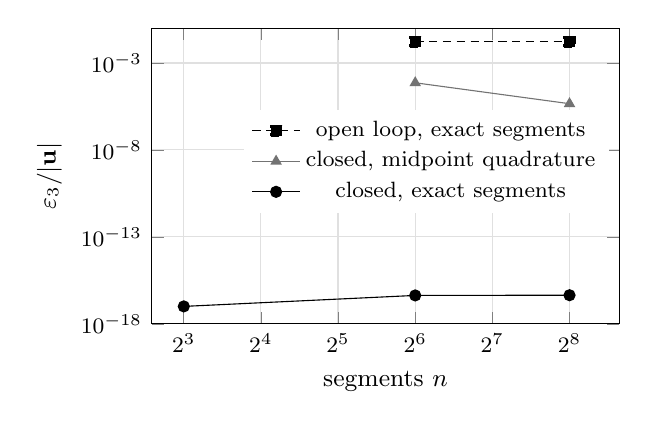
\begin{tikzpicture}
\begin{axis}[
  width=0.62\textwidth, height=0.44\textwidth,
  xlabel={segments $n$}, ylabel={$\eps/|\mathbf{u}|$},
  xmode=log, ymode=log, log basis x=2,
  xmin=6, xmax=400, ymin=1e-18, ymax=1e-1,
  grid=both, grid style={black!12},
  tick label style={font=\footnotesize}, label style={font=\small},
  legend style={font=\footnotesize, at={(0.98,0.55)}, anchor=east, draw=none},
]
\addplot[black, mark=square*, densely dashed]
  coordinates {(64,1.68e-2) (256,1.68e-2)};
\addlegendentry{open loop, exact segments}
\addplot[black!55, mark=triangle*]
  coordinates {(64,7.28e-5) (256,4.56e-6)};
\addlegendentry{closed, midpoint quadrature}
\addplot[black, mark=*]
  coordinates {(8,1e-17) (64,4.28e-17) (256,4.4e-17)};
\addlegendentry{closed, exact segments}
\end{axis}
\end{tikzpicture}
\caption{The discrete residual carries no resolution floor. With exact segment
integration the grade-3 term telescopes, so a closed filament of constant
circulation cancels to round-off at any number of segments --- detected already
at $n=8$, and unaffected by mollification. Midpoint quadrature instead leaves an
$O(h^2)$ floor which would mask a genuine closure violation of comparable size.
Removing one segment separates the closed and open cases by fifteen orders of
magnitude. The closed-exact values are at the round-off level and are plotted at
their measured magnitudes; the $n=8$ point measured exactly zero and is drawn at
the double-precision floor.}
\label{fig:closure}
\end{figure}

\begin{figure}[htbp]
\centering
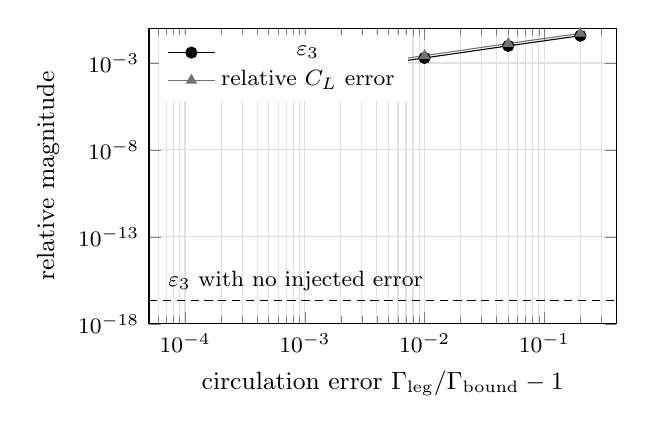
\begin{tikzpicture}
\begin{axis}[
  width=0.62\textwidth, height=0.44\textwidth,
  xlabel={circulation error $\Gamma_{\mathrm{leg}}/\Gamma_{\mathrm{bound}} - 1$},
  ylabel={relative magnitude},
  xmode=log, ymode=log, xmin=5e-5, xmax=0.4, ymin=1e-18, ymax=1e-1,
  grid=both, grid style={black!12},
  tick label style={font=\footnotesize}, label style={font=\small},
  legend style={font=\footnotesize, at={(0.02,0.98)}, anchor=north west,
                draw=none},
]
\addplot[black, mark=*]
  coordinates {(1e-4,1.96e-5) (1e-3,1.96e-4) (1e-2,1.96e-3)
               (5e-2,9.68e-3) (2e-1,3.72e-2)};
\addlegendentry{$\eps$}
\addplot[black!55, mark=triangle*]
  coordinates {(1e-4,2.66e-5) (1e-3,2.66e-4) (1e-2,2.65e-3)
               (5e-2,1.31e-2) (2e-1,5.05e-2)};
\addlegendentry{relative $C_L$ error}
\addplot[black, densely dashed, domain=5e-5:0.4, forget plot] {2.3e-17};
\node[anchor=south west, font=\footnotesize] at (axis cs:6e-5,2.3e-17)
  {$\eps$ with no injected error};
\end{axis}
\end{tikzpicture}
\caption{Detection of a circulation-conservation error in an elliptic-wing
vortex lattice. Within this perturbation family the residual is proportional to
the lift error, the ratio holding to three digits across four decades. The
dashed line is the residual of the unperturbed lattice: a $0.01\%$ circulation
error moves $C_L$ by $\num{2.7e-5}$, which no force-based check would flag, while
lifting $\eps$ twelve orders of magnitude above its clean value.}
\label{fig:detection}
\end{figure}

\begin{figure}[htbp]
\centering
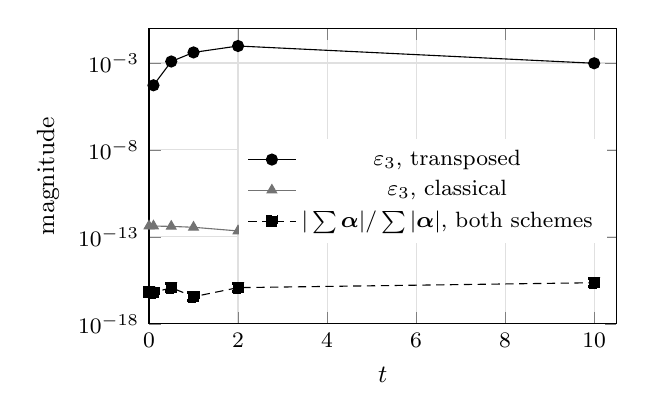
\begin{tikzpicture}
\begin{axis}[
  width=0.62\textwidth, height=0.44\textwidth,
  xlabel={$t$}, ylabel={magnitude}, ymode=log,
  xmin=0, xmax=10.5, ymin=1e-18, ymax=1e-1,
  grid=both, grid style={black!12},
  tick label style={font=\footnotesize}, label style={font=\small},
  legend style={font=\footnotesize, at={(0.98,0.45)}, anchor=east, draw=none},
]
\addplot[black, mark=*]
  coordinates {(0.1,5.22e-5) (0.5,1.22e-3) (1.0,4.06e-3) (2.0,9.50e-3)
               (10.0,9.66e-4)};
\addlegendentry{$\eps$, transposed}
\addplot[black!55, mark=triangle*]
  coordinates {(0,4.19e-13) (0.1,4.18e-13) (0.5,4.00e-13) (1.0,3.56e-13)
               (2.0,2.19e-13) (10.0,3.58e-13)};
\addlegendentry{$\eps$, classical}
\addplot[black, mark=square*, densely dashed]
  coordinates {(0,6.8e-17) (0.1,6.2e-17) (0.5,1.2e-16) (1.0,3.6e-17)
               (2.0,1.2e-16) (10.0,2.3e-16)};
\addlegendentry{$|\sum\balpha|/\sum|\balpha|$, both schemes}
\end{axis}
\end{tikzpicture}
\caption{An emergent violation that no local check can see. An elliptical vortex
ring of 200 particles is advanced under the two standard stretching
discretisations from a common machine-zero start. A material line element obeys
$\dd(\dd\boldsymbol{\ell})/\dd t = (\dd\boldsymbol{\ell}\cdot\nabla)\bu$, which is
the classical scheme, so a filament-derived particle set retains its structure
under it. The transposed scheme drifts ten orders of magnitude within a tenth of
a time unit. Throughout, the conservation check a practitioner would normally
rely on sits at machine precision for both schemes and detects nothing.}
\label{fig:vpm}
\end{figure}


\subsection{Filament closure}

Table~\ref{tab:filament} and Figure~\ref{fig:closure} evaluate the residual on a
fixed asymmetric, non-planar closed curve. Closed and open are separated by
fifteen orders of magnitude, closure is detected exactly at eight segments, and
mollification does not degrade it. The midpoint rows show the $O(h^2)$ floor
that Theorem~\ref{thm:Bprime} removes.

\begin{table}[htbp]
\centering
\caption{Relative residual $\eps/|\bu|$ on an asymmetric closed curve,
$\Gamma=1.7$.}
\label{tab:filament}
\begin{tabular}{lr}
\toprule
Configuration & $\eps/|\bu|$ \\
\midrule
Closed, exact segments, $n=8$ & \num{0.0} \\
Closed, exact segments, $n=64$ & \num{4.28e-17} \\
Closed, exact segments, $n=64$, $\delta=0.1$ & \num{4.33e-17} \\
Closed, midpoint quadrature, $n=64$ & \num{7.28e-5} \\
Closed, midpoint quadrature, $n=256$ & \num{4.56e-6} \\
Open (one segment removed), exact, $n=64$ & \num{1.68e-2} \\
Closed, $\Gamma$ varying along the loop, exact & \num{7.03e-3} \\
\bottomrule
\end{tabular}
\end{table}

\subsection{A circulation-conservation error}
\label{sec:injected}

Scaling trailing-leg circulation off bound circulation by a fixed ratio violates
Helmholtz's second theorem. It is a routine implementation slip and it leaves a
plausible lift coefficient behind.

\begin{table}[htbp]
\centering
\caption{Injected circulation error, elliptic wing, $AR=8$, $\alpha=5^\circ$,
80 spanwise stations.}
\label{tab:injected}
\begin{tabular}{lrrrr}
\toprule
$\Gamma_{\text{leg}}/\Gamma_{\text{bound}}$ & $C_L$ & Rel.\ $C_L$ error & $\eps$ & $\eps/\text{error}$ \\
\midrule
$1.0000$ & $0.41894$ & ---           & \num{2.3e-17} & --- \\
$1.0001$ & $0.41893$ & \num{2.66e-5} & \num{1.96e-5} & $0.738$ \\
$1.0010$ & $0.41883$ & \num{2.66e-4} & \num{1.96e-4} & $0.738$ \\
$1.0100$ & $0.41783$ & \num{2.65e-3} & \num{1.96e-3} & $0.738$ \\
$1.0500$ & $0.41344$ & \num{1.31e-2} & \num{9.68e-3} & $0.738$ \\
$1.2000$ & $0.39778$ & \num{5.05e-2} & \num{3.72e-2} & $0.736$ \\
\bottomrule
\end{tabular}
\end{table}

Figure~
ef{fig:detection} shows the result. Two observations. Within this
perturbation family the residual is proportional to the lift error, the ratio holding to three digits across four decades. And a
$0.01\%$ circulation error moves $C_L$ by $\num{2.7e-5}$ --- which no
force-based check would flag --- while lifting $\eps$ twelve orders of magnitude
above its clean value.

The constant of proportionality is not universal: the wing--body configuration
of Section~\ref{sec:mixed} gives $0.042$, equally stable across decades. The
claim is proportionality within a perturbation family for a given
configuration, together with detection far below the noise floor of any
force-based check --- not a calibration-free error estimate.

\subsection{Truncated wakes}

Cutting trailing legs at finite distance $L$ leaves a topologically open
filament. Detection is absolute, fifteen orders between open and closed at the
same $L$, but the residual decays as $L^{-3}$ while the lift error decays as
$L^{-2}$, so it is not a proxy for force error in this failure mode. Both
exponents should be reported: the diagnostic detects the violation without
quantifying its aerodynamic consequence.

\subsection{Mixed fields}
\label{sec:mixed}

Corollary~\ref{cor:blind} is exercised on a wing--body configuration in which
fuselage source panels (scalar grade) and wing horseshoe circulations (bivector
grade) are unknowns in one linear system, the influence matrix assembled column
by column from the same kernel. The physics is recovered correctly: holding the
wing lattice identical and varying only the fuselage, lift carryover rises
monotonically ($+0.81\%$, $+3.21\%$, $+7.28\%$, $+13.74\%$ for fuselage radii
$0.2$ to $0.8$) while root circulation increases from $0.1138$ to $0.1521$ and
tip circulation is essentially unchanged. Throughout, with several hundred
source panels active, $\eps$ remains at $\sim\!\num{6e-18}$ and the injected
error experiment proceeds unaffected. The diagnostic requires no modification to
operate inside a source-dominated problem.

% =====================================================================
\section{Dynamic detection}
\label{sec:dynamic}

The failure modes above, although realistic, are all catchable by an assertion
on the element data. Solenoidality loss in a particle method is not: it is
generated by the stretching term, every particle strength remains individually
valid, and there is no local invariant to test.

\begin{table}[htbp]
\centering
\caption{Solenoidality drift, elliptical ring, 200 particles. $\eps$ is RMS over
particles normalised by RMS speed; closure is $|\sum\balpha|/\sum|\balpha|$.}
\label{tab:vpm}
\begin{tabular}{lrrrr}
\toprule
& \multicolumn{2}{c}{$\eps$} & \multicolumn{2}{c}{Closure} \\
\cmidrule(lr){2-3}\cmidrule(lr){4-5}
$t$ & Classical & Transposed & Classical & Transposed \\
\midrule
$0$    & \num{4.19e-13} & \num{4.19e-13} & \num{6.8e-17} & \num{6.8e-17} \\
$0.1$  & \num{4.18e-13} & \num{5.22e-5}  & \num{6.2e-17} & \num{3.5e-17} \\
$0.5$  & \num{4.00e-13} & \num{1.22e-3}  & \num{1.2e-16} & \num{5.3e-17} \\
$1.0$  & \num{3.56e-13} & \num{4.06e-3}  & \num{3.6e-17} & \num{1.1e-16} \\
$2.0$  & \num{2.19e-13} & \num{9.50e-3}  & \num{1.2e-16} & \num{1.0e-16} \\
$10.0$ & \num{3.58e-13} & \num{9.66e-4}  & \num{2.3e-16} & \num{7.8e-17} \\
\bottomrule
\end{tabular}
\end{table}

Table~\ref{tab:vpm} and Figure~\ref{fig:vpm} follow an elliptical vortex ring under the two standard
stretching discretisations. A material line element obeys
$\dd(\dd\boldsymbol{\ell})/\dd t = (\dd\boldsymbol{\ell}\cdot\nabla)\bu$, which
is the classical scheme, so a filament-derived particle set retains its
structure under it while the transposed scheme does not.

The two right-hand columns are the point. The conservation check sits at machine
precision for both schemes at every time and is completely blind. The residual
separates them by ten orders of magnitude, from a common machine-zero start,
purely through the dynamics. This bears on practice, since the transposed scheme
is the default in current solvers, applied with Pedrizzetti relaxation precisely
to control the divergence it generates \cite{alvarez2024,pedrizzetti1992}. The
scope is narrow: the transposed scheme fails to preserve solenoidality
\emph{for filament-derived particle sets}, and its conservation advantages for
volumetric fields are not in question.

\subsection{Independent validation of the mechanism}

Table~\ref{tab:vpm} is a statement about published schemes measured with the
diagnostic this paper proposes, so we verify its mechanism twice more without
using $\eps$.

In an imposed linear velocity field $\bu = A\bx$ the Jacobian is the constant
$A$, and Cauchy's vorticity formula makes $\balpha(t) = e^{At}\balpha(0)$ exact.
Halving the step, the classical scheme gives relative errors $\num{1.40e-4}$,
$\num{3.54e-5}$, $\num{8.93e-6}$, $\num{2.24e-6}$ --- clean second order, the
time integrator's own accuracy --- while the transposed scheme gives $1.3396$,
$1.3400$, $1.3401$, $1.3402$. The transposed error does not converge because it
is not a discretisation error but a different equation, whenever $A$ has an
antisymmetric part.

Separately, on the ring itself $\bx_{k+1}-\bx_{k-1}$ is a material line element
regardless of how strengths evolve, since positions are advected by the flow.
Frozen vorticity requires $\balpha_k$ to remain parallel to it and proportional
in length. Departure from parallelism reaches $\num{2.6e-8}$ under the classical
scheme against $\num{6.5e-4}$ under the transposed one, with stretch errors
$\num{3.2e-4}$ against $\num{1.4e-2}$.

Both checks take their reference from a known analytic solution or from particle
trajectories rather than from the diagnostic. Neither is a new result --- it is
the textbook distinction between the two discretisations --- which is precisely
why it serves as validation of the implementation.

\subsection{Grading the defect}

The residual measures how far a particle set is from representing a solenoidal
field, not merely whether it is. Displacing particles off the curve by a
fraction of the core radius, strengths untouched, gives $\eps = \num{7.09e-3}$,
$\num{3.37e-2}$, $\num{9.77e-2}$ for jitter amplitudes $0.02\delta$,
$0.1\delta$, $0.5\delta$: linear in the perturbation and roughly $27\times$ more
sensitive than the closure check at small amplitude.

% =====================================================================
\section{An open question: relaxation}
\label{sec:relaxation}

Relaxation is applied on a fixed schedule because the drift it corrects has not
been observable. A free measurement makes its effect an empirical question. We
report two experiments in opposite regimes and draw a limited conclusion.

In the filament-derived case, Pedrizzetti relaxation applied every step at
strength $f$ gives $\eps = \num{9.66e-4}$ at $f=0$ against $\num{1.70e-2}$,
$\num{2.16e-2}$ and $\num{8.40e-3}$ at $f = 0.02, 0.05, 1.0$, with impulse drift
rising from $\num{3.9e-5}$ to $\num{1.4e-2}$. Every strength worsens both
measures. The recovered vorticity is sound --- the mean of
$\cos(\balpha,\bomega)$ is $0.999979$ initially and $0.999829$ at $t=10$, so the
realignment is nearly a null operation --- and its cumulative effect is
nonetheless adverse. This is unsurprising: a set lying on a curve with exact
tangents is already solenoidal to round-off, and a corrective scheme applied to
a healthy field can only do harm.

We therefore built the opposite regime. Vorticity is laid on a Cartesian
lattice through a ring core with a Gaussian profile, making the initial
divergence a genuine $O(h^2)$ discretisation error rather than zero, and two
coaxial rings are leapfrogged to sustain stretching. Here the sign reverses:
$\eps$ falls from $\num{1.98e-2}$ at $f=0$ to $\num{1.53e-2}$ at $f=0.2$, some
$23\%$, with a shallow optimum near $f\approx0.05$--$0.2$ and a return to
$\num{1.96e-2}$ at $f=1$. Impulse drift worsens from $\num{1.4e-3}$ to
$\num{4}$--$\num{7e-3}$ over the same range.

Neither experiment settles the matter and we do not present them as doing so.
The volumetric setup fails its own validation: measured ring translation speed
is $18\%$ below Saffman's value at the finest resolution reached, improving only
slowly through $-27\%$, $-21\%$, $-18\%$ as $h$ falls. The cause is structural.
Blob overlap requires $\delta\approx1.3h$ while faithful representation of the
physical core requires $\delta\ll a$; at particle counts direct summation
permits these cannot hold together, and $\delta/a = 0.65$ in the finest case, so
smoothing dominates the core the ring is meant to have. Refining $h$ moreover
shrinks $\delta$ with it, confounding the study. A $23\%$ reduction that is
non-monotone in $f$, obtained in a configuration mis-predicting a basic integral
quantity, supports no claim either way.

What the pair does establish is that the effect is regime-dependent with
opposite signs, so results from either alone would mislead. The methodological
point stands independently: the effectiveness of relaxation is now measurable
per configuration at no cost, where previously it could only be inferred from
stability. Deciding it requires resolutions at which $\delta\ll a$ and
$\delta\gtrsim h$ hold simultaneously, of order $10^4$--$10^5$ particles, which
places the question beyond direct summation. Fast summation is therefore a
prerequisite for answering it rather than an optimisation, and we address it in
a companion study.

% =====================================================================
\section{Scope and limitations}
\label{sec:scope}

The most important limitation is one of interpretation. A vanishing residual
certifies that a discrete vortex system is a \emph{realisable} vorticity field;
it does not certify accuracy. In the wake-truncation study the configurations
with a closing starting vortex have $\eps$ at round-off and are simultaneously
the least accurate entries: a closed wake at half a span is the honest field of
an impulsively started wing at early time, not a poor approximation of the
steady one. The diagnostic answers ``is this a realisable vortex system?'',
never ``is this the right answer?''.

Three further limits. The proportionality constant between $\eps$ and force
error is configuration-dependent and must be calibrated per problem for a
quantitative estimate. Exact segment integration is required for the floor-free
property of Theorem~\ref{thm:Bprime}. And the present work is steady,
incompressible and inviscid at the level of the boundary-integral solvers; the
extension to unsteady compressible flow is the same construction in the
spacetime algebra $Cl(1,3)$, where the corresponding Dirac operator yields
retarded kernels.

% =====================================================================
\section{Conclusions}

The grade-3 part of the Clifford velocity kernel, discarded by every
implementation because the cross-product formulation never forms it, is the
Newtonian potential of the vorticity divergence. Integrated exactly along
straight segments it carries no discretisation floor and so measures topology
rather than resolution; it is blind to source content by construction; and it
costs one inner product of quantities already in registers, surviving fast
summation because it emerges from the same local expansion as the velocity.

It detects a $0.01\%$ circulation-conservation error twelve orders of magnitude
above its noise floor while the lift coefficient moves by $\num{2.7e-5}$, and on
an evolving particle ring it separates two standard stretching discretisations
by ten orders of magnitude while the conservation check normally relied upon
detects nothing. Solenoidality loss in vortex particle methods is presently
corrected by schemes whose effectiveness is inferred from stability rather than
measured. Whether that practice can be improved is not settled here, and the
resolution required to settle it is identified; the contribution of this paper
is that the measurement is now available at no cost.

\section*{Reproducibility}

The implementation, verification suite and all reported tables are available at
\texttt{[repository URL]}.

% =====================================================================
\begin{thebibliography}{99}

\bibitem{alvarez2024}
E.~J. Alvarez, A.~Ning,
Stable vortex particle method formulation for meshless large-eddy simulation,
AIAA Journal (2024). [VERIFY volume/pages]

\bibitem{cottet2000}
G.-H. Cottet, P.~D. Koumoutsakos,
Vortex Methods: Theory and Practice,
Cambridge University Press, 2000.

\bibitem{doran2003}
C.~Doran, A.~Lasenby,
Geometric Algebra for Physicists,
Cambridge University Press, 2003.

\bibitem{greengard1987}
L.~Greengard, V.~Rokhlin,
A fast algorithm for particle simulations,
Journal of Computational Physics 73 (1987) 325--348.

\bibitem{gurlebeck1997book}
K.~Gürlebeck, W.~Sprößig,
Quaternionic and Clifford Calculus for Physicists and Engineers,
Wiley, 1997.

\bibitem{hessmith1967}
J.~L. Hess, A.~M.~O. Smith,
Calculation of potential flow about arbitrary bodies,
Progress in Aerospace Sciences 8 (1967) 1--138.

\bibitem{hestenes1984}
D.~Hestenes, G.~Sobczyk,
Clifford Algebra to Geometric Calculus,
Reidel, 1984.

\bibitem{katzplotkin2001}
J.~Katz, A.~Plotkin,
Low-Speed Aerodynamics, 2nd Edition,
Cambridge University Press, 2001.

\bibitem{pedrizzetti1992}
G.~Pedrizzetti,
Insight into singular vortex flows,
Fluid Dynamics Research 10 (1992) 101--115. [VERIFY]

\bibitem{saffman1992}
P.~G. Saffman,
Vortex Dynamics,
Cambridge University Press, 1992.

\bibitem{sprossig1997}
W.~Sprößig, K.~Gürlebeck,
On the treatment of fluid problems by methods of Clifford analysis,
Mathematics and Computers in Simulation 44 (1997). [VERIFY pages]

\bibitem{sugon2024}
Fluid Maxwell's equations in the language of geometric algebra,
Pramana --- Journal of Physics (2024). [VERIFY authors, volume, pages]

\bibitem{vanoosterom1983}
A.~van Oosterom, J.~Strackee,
The solid angle of a plane triangle,
IEEE Transactions on Biomedical Engineering 30 (1983) 125--126.

\bibitem{winckelmans1993}
G.~S. Winckelmans, A.~Leonard,
Contributions to vortex particle methods for the computation of
three-dimensional incompressible unsteady flows,
Journal of Computational Physics 109 (1993) 247--273.

\end{thebibliography}

\end{document}
